\RequirePackage{luatex85}
\documentclass{standalone}
\usepackage{tikz}
\usetikzlibrary{shapes.geometric}


\begin{document}
\begin{tikzpicture}
\node[] at (0,0) {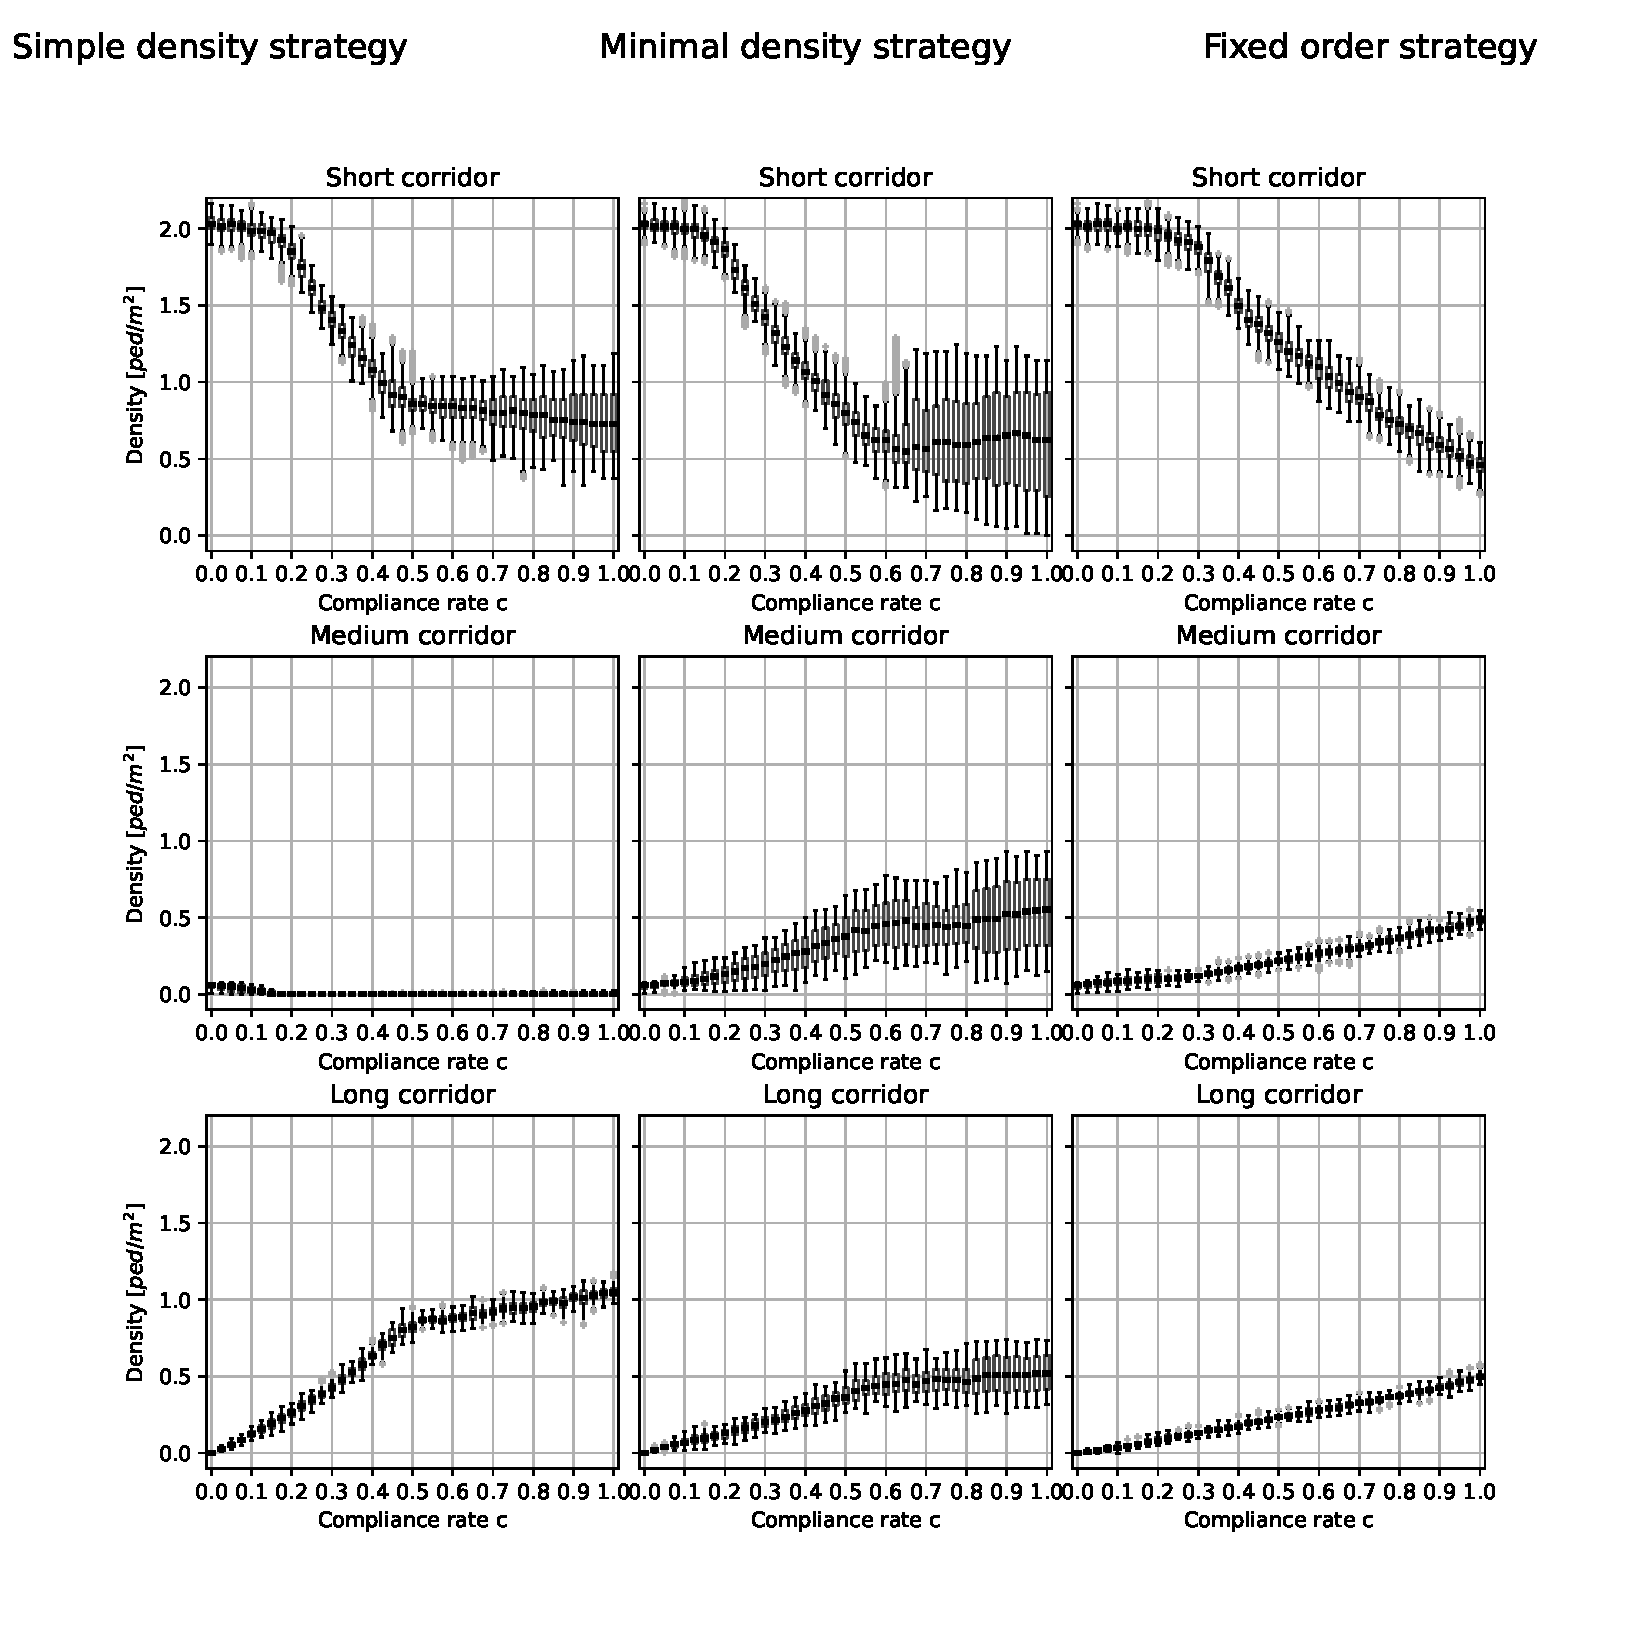
\includegraphics[width=16cm,trim={1.5cm 1cm 1cm 2.7cm}, clip]{densities.pdf} };
\node[] at (-4.5,8) {Simple density alg. };
\node[] at (0,8) {Minimal density alg. };
\node[] at (4.5,8) {Alternating alg. };
\draw[red,dashed] (-5.8,3.5) -- (-5.8,7.2);
\draw[red,dashed] (-4.55,3.5) -- (-4.55,7.2);
\draw[red,dashed] (-1.2,3.5) -- (-1.2,7.2);
\draw[red,dashed] (0.5,3.5) -- (0.5,7.2);
\draw[red,dashed] (3.8,3.5) -- (3.8,7.2);
\node[fill=gray,text width=0.6cm] at (-6.3,5.3) {\footnotesize{Jam-ming}};
\node[fill=gray,text width=0.6cm] at (-1.7,5.3) {\footnotesize{Jam-ming}};
\node[fill=gray,text width=0.6cm] at (3.2,5.3) {\footnotesize{Jam-ming}};

\node[fill=gray,text width=1.4cm] at (-3.2,6.5) {\footnotesize{Compensa-tion}};
\node[fill=gray,text width=1.4cm] at (1.5,6.5) {\footnotesize{Compensa-tion}};


\node[fill=blue!50,text width=3.2cm] at (-4.3,1.6) {\footnotesize{This alg. never recommends the medium route}};


\node[text width=3.8cm] at (-4.5,-0.1) {\footnotesize{caused by agents queuing in front of the short route}};

\draw[orange] (-6.5,-1.2) circle (0.5);

\end{tikzpicture}

\end{document}